%% PODSTAWOWE USTAWIENIA DOKUMENTU
\documentclass[12pt, a4paper, polish]{article}
\DeclareUnicodeCharacter{2003}{-}
%\usepackage[a4paper, lmargin=2.5cm, rmargin=2.5cm, hmargin=2.5cm, bmargin=2.5cm]{geometry}
\usepackage[a4paper,top=2.5cm,bottom=1.5cm,left=1.5cm,right=1.5cm]{geometry}
%\geometry{verbose,lmargin=2.5cm,rmargin=2.5cm}
\usepackage{enumerate}
% Symbole matematyczne
\usepackage{latexsym}
% Formatowanie czcionki
\usepackage[T1]{fontenc}
% Formatowanie polskich znaków
\usepackage{polski}
\usepackage[utf8]{inputenc}
% Akapit po sekcji
%\usepackage{indentfirst}
% Ustawienie nagłówków i stopek
\usepackage{fancyhdr}
% Liczba stron
\usepackage{lastpage}
% Kolumny
\usepackage{paracol}
% Czcionka latin modern
\usepackage{lmodern}
% Równania matematyczne
\usepackage{amsmath}
\usepackage{amsfonts}
\usepackage{amssymb}
\usepackage{amsthm}
% Wstawianie grafik
\usepackage{graphicx}
\usepackage[section]{placeins} % Ogarnięcie obrazków
\usepackage{float}
\usepackage{subcaption}
%\usepackage[outdir=./]{epstopdf}
\usepackage{grffile}

%% ODSTĘPY W WIERSZACH
\setlength{\parindent}{1.2cm}
\setlength{\parskip}{0.05cm}
\linespread{1}

%% SZARE TŁO TEKSTU
\usepackage[most]{tcolorbox}
\tcbset{
	frame code={}
	center title,
	left=0pt,
	right=0pt,
	top=0pt,
	bottom=0pt,
	colback=gray!30,
	colframe=white,
	width=\dimexpr\textwidth\relax,
	enlarge left by=0mm,
	boxsep=5pt,
	arc=0pt,outer arc=0pt,
}

% HIPERŁĄCZA SPISU TREŚCI
\usepackage{hyperref}
\hypersetup{
	colorlinks,
	citecolor=black,
	filecolor=black,
	linkcolor=black,
	urlcolor=black
}

\begin{document}
	\fancyhf{}	% Usunięcie domyślnego stylu numerowania
	
	% ********************** TYTUŁ ****************************
	\noindent\textsf{\begin{Large}Laboratorium Sterowania Robotów Manipulacyjnych \\\end{Large}
		Raport z ćwiczeń\textbf{ Z7, Z8}\\
		Szymon Kacperek, Adrianna Kręglewska, Adam Banaszczyk\\
		AiR, studia stacjonarne II stopnia,  specjalność SSiR, rok akademicki 2019/2020\\
		\rule{\columnwidth}{0.2pt}}
	
	\thispagestyle{empty}
	\pagestyle{fancy}
	\fancyhead{}
	\rhead{\thepage}
	\renewcommand{\headrulewidth}{0pt}%{}
	\setlength{\footskip}{1mm}
	
	%							*****************POCZĄTEK DOKUMENTU*****************
	\section{Sterowanie w podprzestrzeni typu \textit{hiperkula}}
	Dla modelu manipulatora PM2R z silnikami zaprojektowany został regulator ROOS dla ograniczonej podprzestrzeni sterowań: hiperkuli. Układ sterowania wyrażony jest wprost dla napięć wraz ze wzmacniaczem mocy, ograniczającym napięcia zasilania dla obu silników. Symulacje przebiegają dla zerowych warunków początkowych (manipulator wyprostowany w prawo).
	
	Z założeń wynika, iż regulator ROOS jest odporny na nieznajomość strukturalną i parametryczną modelu, zatem dla celów symulacji wprowadzono niepewności parametryczne: 10\% dla długości pierwszego oraz drugiego ramienia oraz 10\% dla masy drugiego ramienia. Silnik został zamodelowany według danych \textit{maxon DC motor FF2260, 883} oraz dwóch przekładni \textit{110507} o przełożeniu $\eta=1/181$. Wartości współczynników diagonalnych macierzy wzmocnie dla $\epsilon=0,9$ przyjęto eksperymentalnie oraz ograniczono napięcia zasilania aktuatorów:
	\begin{equation}\label{eqn:regulatory}
	\Lambda=\begin{bmatrix} 2,3 & 0 \\0 & 2,2 \end{bmatrix}, \quad  
	D=\begin{bmatrix} 0,05 & 0 \\0 & 0,05 \end{bmatrix}, \quad 
	u_{max}=\begin{bmatrix}24 \\ 24 \end{bmatrix}[V]
		\end{equation}
	Podstawowym ograniczeniem podprzestrzeni typu \textit{hiperkula} jest ograniczenie napięcia sterującego $u_{HKmax}=\min\{u_{max}\}$. Efekt ograniczenia widoczny jest na rys. \ref{fig:hiperkula12v}. W przypadku nierównych napięć zasilania, sygnał sterujący bazuje na najmniejszym z ograniczeń, zwiększając czas ustalania odpowiedzi układu, maksymalny moment napędowy. W takiej konfiguracji, zmieniając doświadczalnie napięcie zasilania $\tau_{1max}$, do wartości $\overline{\tau_{1max}}= 16$ [V], przebieg uchybu przestał zbiegać asymptotycznie do otoczenia zera. 

	\subsection{Prezentacja wyników}
	\begin{figure}[h]
		\centering	
		a) 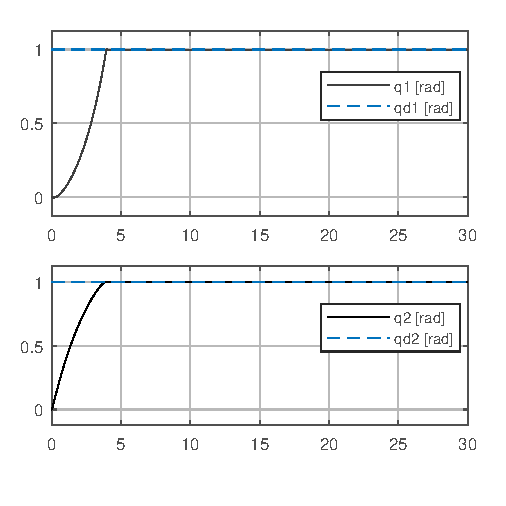
\includegraphics[width=0.30\columnwidth]{SRManL4_ZADANIE1/figs/01Pozycje_U12} b)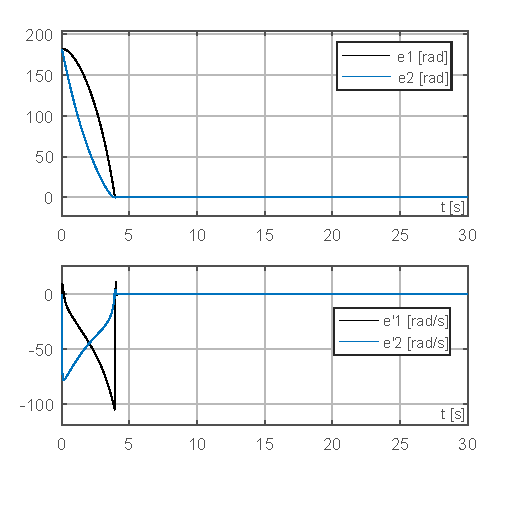
\includegraphics[width=0.30\columnwidth]{SRManL4_ZADANIE1/figs/01Uchyby_U12} c)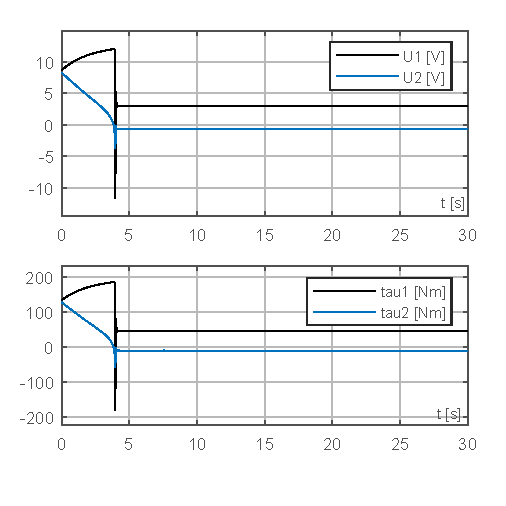
\includegraphics[width=0.30\columnwidth]{SRManL4_ZADANIE1/figs/01Sygnaly_U12}\caption{
			Wyniki symulacji dla zmniejszonego napięcia zasilania $u_{2max}=12$ [V] o wymuszeniu $Q_d=[1\quad1]$: przebiegi a) pozycji ogniw wraz z zadanym sygnałem referencyjnym, b) uchybów pozycji i prędkości, c)  napięć sterujących oraz odpowiadające im momenty generowane na wałach silników.}\label{fig:hiperkula12v}
	\end{figure}
	\begin{figure}[!ht]\centering
		a) 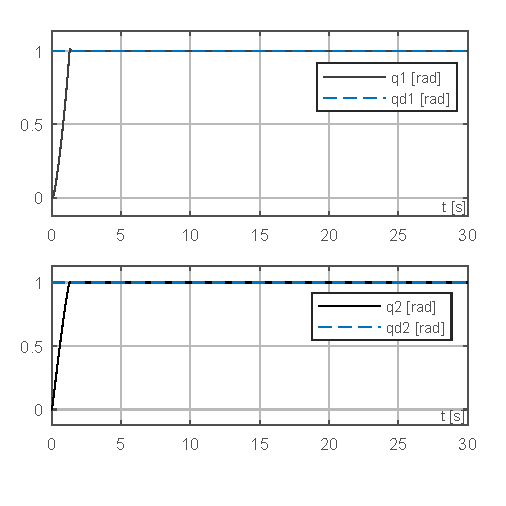
\includegraphics[width=0.30\columnwidth]{SRManL4_ZADANIE1/figs/02Pozycje_U24} b)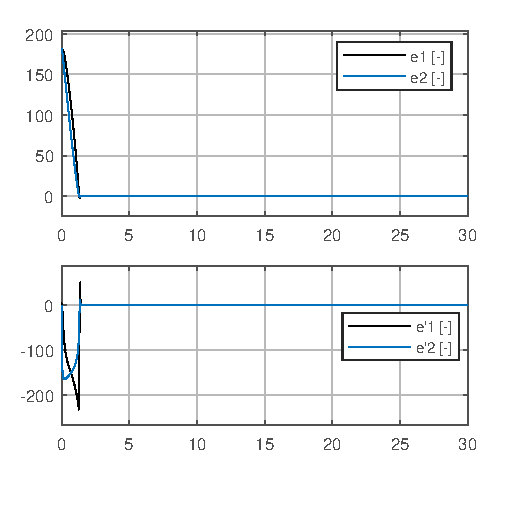
\includegraphics[width=0.30\columnwidth]{SRManL4_ZADANIE1/figs/02Uchyby_U24} c)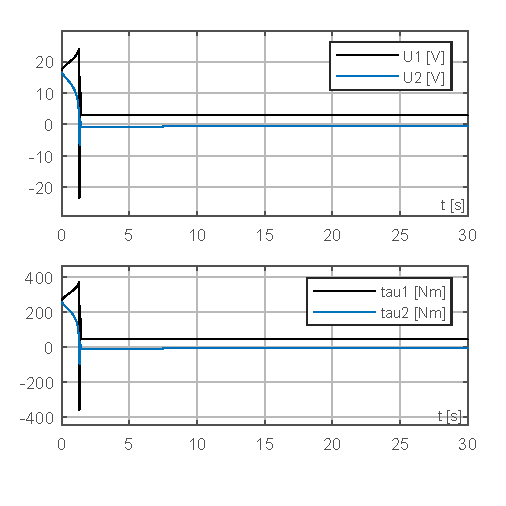
\includegraphics[width=0.30\columnwidth]{SRManL4_ZADANIE1/figs/02Sygnaly_U24}\\
		d) 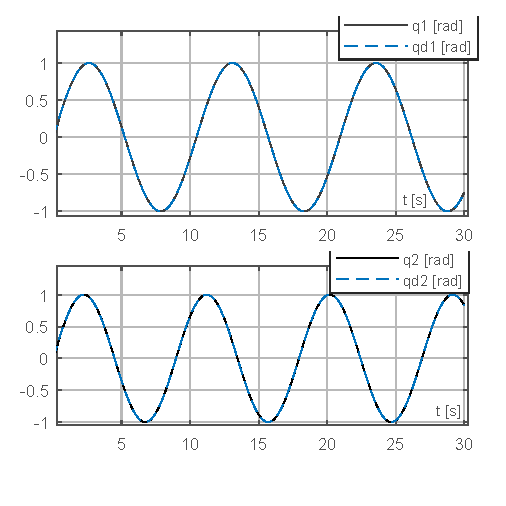
\includegraphics[width=0.30\columnwidth]{SRManL4_ZADANIE1/figs/03Pozycje_U24} e)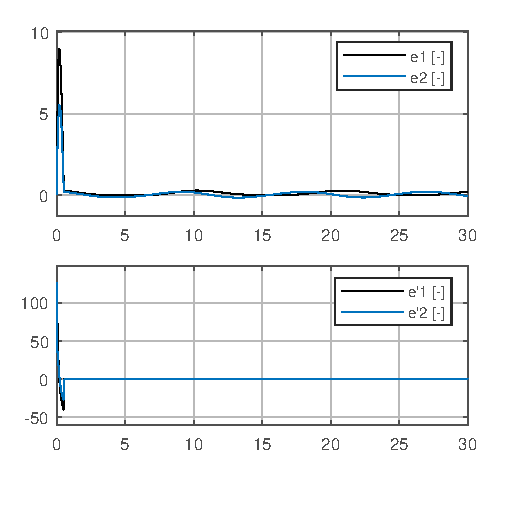
\includegraphics[width=0.30\columnwidth]{SRManL4_ZADANIE1/figs/03Uchyby_U24} f)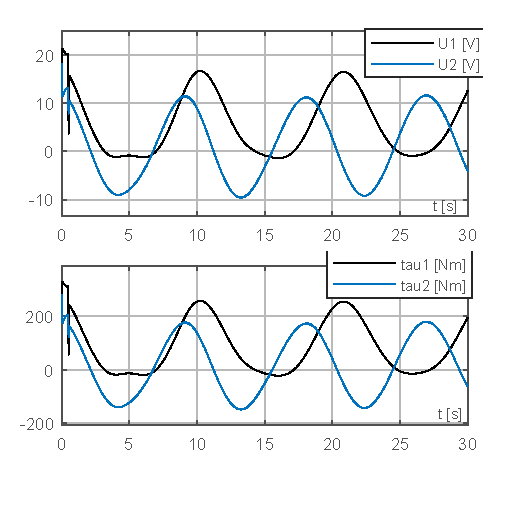
\includegraphics[width=0.30\columnwidth]{SRManL4_ZADANIE1/figs/03Sygnaly_U24}\\
		g) 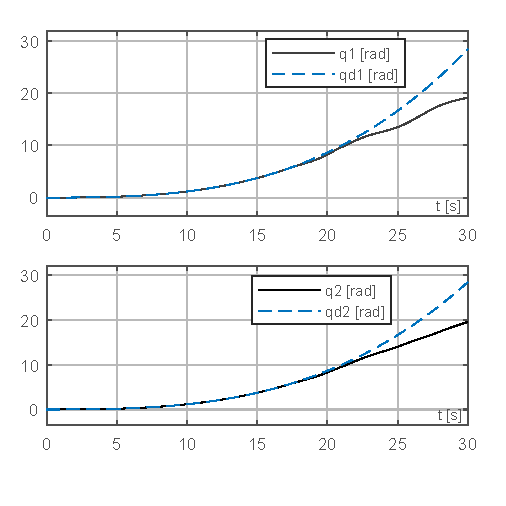
\includegraphics[width=0.30\columnwidth]{SRManL4_ZADANIE1/figs/04Pozycje_U24} h)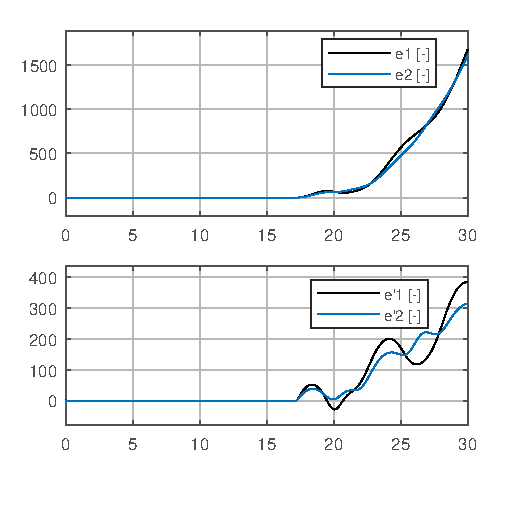
\includegraphics[width=0.30\columnwidth]{SRManL4_ZADANIE1/figs/04Uchyby_U24} i)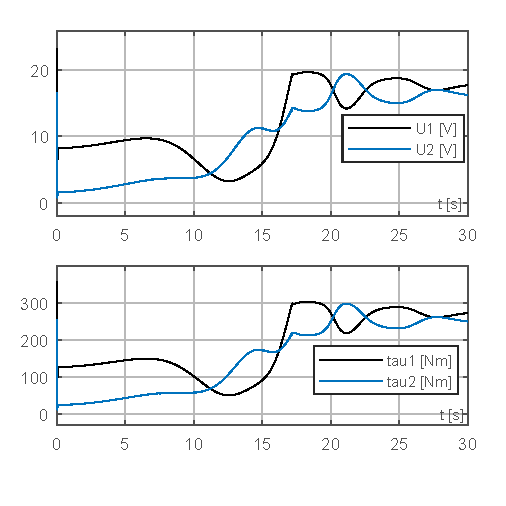
\includegraphics[width=0.30\columnwidth]{SRManL4_ZADANIE1/figs/04Sygnaly_U24}\caption{
			Wyniki symulacji dla $u_{HKmax}=24$ [V]. Przebiegi (a, d, g) pozycji ogniw wraz z zadanym sygnałem referencyjnym, (b, e, h) uchybów pozycji i prędkości, (c, f, i)  napięć sterujących oraz odpowiadające im momenty generowane na wałach silników, o wymuszeniu:\\
			\textbf{a-c:} $Q_{d1}=[1\quad1]$;\\
			\textbf{d-f:} $Q_{d2}=[\sin(0,6t);\quad \sin(0,7t)]$;\\
			\textbf{g-i:} $Q_{d3}=[0,0025t^3+0,0020t^2+0,0015t+0,001]$.}
	\end{figure}
		
	\subsection{Wnioski}
	Z obserwacji wynika, iż zjawisko \textit{chatteringu} staje się intensywniejsze, gdy wartość współczynnika $\epsilon$ maleje. Dla dobranych nastaw (\ref*{eqn:regulatory}) występują miejscowe \textit{peaki} o wartości ok. $0,15 [V]$. Przyjmując za $\epsilon=0$, zjawisko znacznie się intensyfikuje, oscylując między granicznymi wartościami napięć sterujących z wysoką częstotliwością. Uniemożliwia to poprawne sterowanie obiektem i może doprowadzić do zniszczenia części mechanicznych.  
	
	Dla wymuszenia $Q_{d1}$ błędy śledzenia zbiegają do wartości ok. $e_1=0,04$ oraz $e_2=-0,01$. i ich wartość jest zależna od współczynnika $\epsilon$ - im jest większy, tym błędy śledzenia rosną. Dla wymuszenia $Q_{d3}$ wartości uchybów również zbiegają asymptotycznie do zera, aż do momentu, gdy sygnał referencyjny pozycji zadanej rośnie zbyt szybko, by manipulator mógł nadążyć. Dla wymuszenia $Q_{d2}$, błędy śledzenia oscylują wokół zera, tworząc tunel.
	
	Dla wymuszenia $Q_{d1}$, zmniejszając napięcie zasilania do $\overline{u_{1max}}=16[V]$ błędy śledzenia przestały zbiegać do zera.
	
	Mimo niepewności parametrycznej, odpowiedź modelu manipulatora odwzorowuje zadane wartości referencyjne. Kluczowym ograniczeniem jest zmniejszenie maksymalnej wartości sterowania w przypadku wystąpienia dwóch różnych napięć zasilających aktuatory - prowadzi to do zwiększenia czasu ustalenia odpowiedzi manipulatora oraz ogranicza możliwości sterowania.
	
	\section{Sterowanie w podprzestrzeni typu \textit{hiperprostopadłościan}}
	Podstawowym założeniem sterowania w podprzestrzeni typu \textit{hiperprostopadłościan} jest usunięcie ograniczenia wynikającego z doboru minimalnej wartości $u_{max}$. Regulator ma zapewnić lepszą jakość sterowania, w przypadku wystąpienia różnych napięć zasilających aktuatory. Symulacje przebiegają z identycznymi nastawami regulatorów (\ref{eqn:regulatory}). 
	
	\subsection{Wnioski}
	Błędy śledzenia w przypadku wymuszenia skokowego (rys. 4b) zmierzają asymptotycznie do zera. Jakość sterowania, w tym przypadku, jest identyczna dla obu podprzestrzeni. Różnica wynika natomiast po ograniczeniu napięcia sterującego: $u_{2max}=12$ V, wartość sterowania nie uległa zmniejszeniu jak w przypadku regulatora ROOS w podprzestrzeni typu \textit{hiperkula} (rys. \ref{fig:hiperkula12v}c, rys. \ref{fig:hiperprostopadloscian12v}c). 
	
	Zmniejszenie wartości napięcia zasilania do $\overline{u_{1max}}=16[V]$ w przypadku podprzestrzeni typu \textit{hiperprostopadłościan} spowodowało, iż błędy śledzenia zbiegały asymptotycznie do zera w odróżnieniu do podprzestrzeni typu \textit{hiperkula}. Czas ustalania się odpowiedzi manipulatora uległ wydłużeniu.
	
	Podsumowując, zmiana podprzestrzeni pozwala uniknąć zasadniczej wady. Manipulator może wykorzystać pełne możliwości zainstalowanych aktuatorów.
	
	\subsection{Prezentacja wyników}
	\begin{figure}[h]\centering
		a) 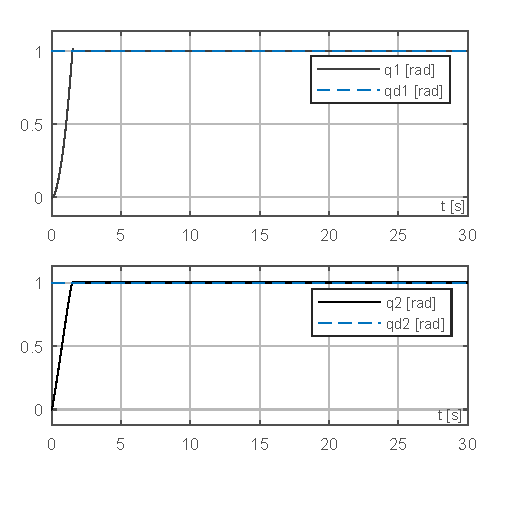
\includegraphics[width=0.30\columnwidth]{SRManL4_ZADANIE2/figs/01Pozycje_U12} b)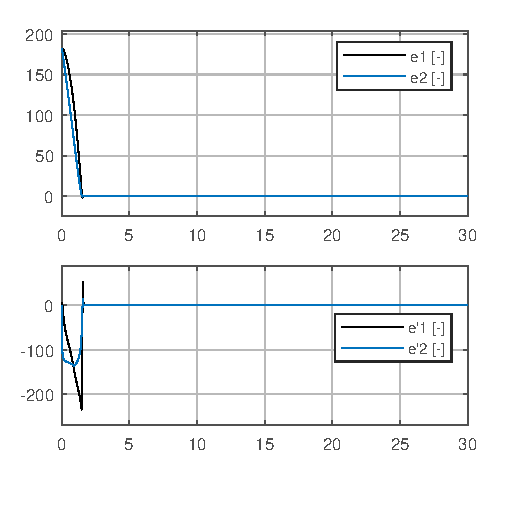
\includegraphics[width=0.30\columnwidth]{SRManL4_ZADANIE2/figs/01Uchyby_U12} c)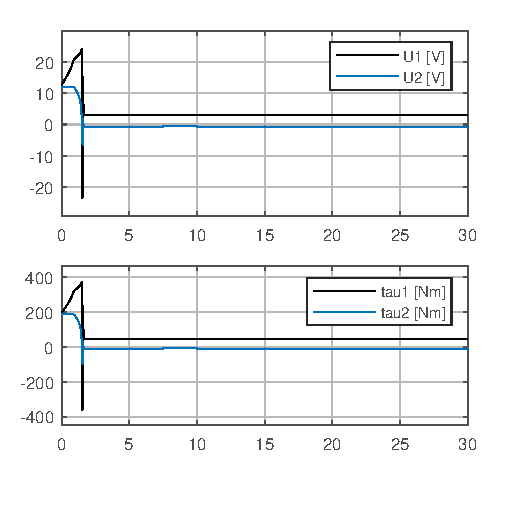
\includegraphics[width=0.30\columnwidth]{SRManL4_ZADANIE2/figs/01Sygnaly_U12}\caption{
			Wyniki symulacji dla $u_{2max}=12$ [V] o wymuszeniu $Q_d=[1\quad1]$: przebiegi a) pozycji ogniw wraz z zadanym sygnałem referencyjnym, b) uchybów pozycji i prędkości, c)  napięć sterujących oraz odpowiadające im momenty generowane na wałach silników.}\label{fig:hiperprostopadloscian12v}
	\end{figure}
	\begin{figure}[H]\centering
		a) 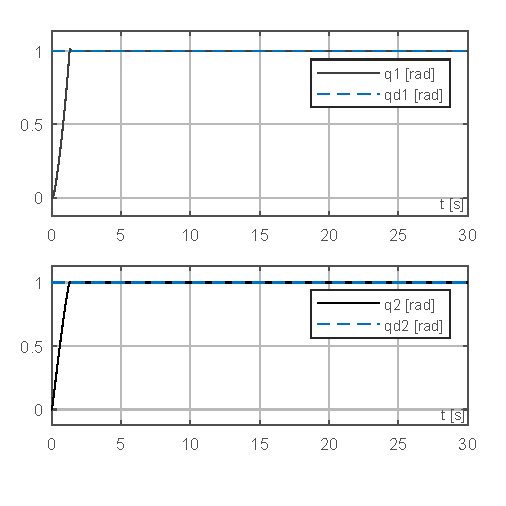
\includegraphics[width=0.30\columnwidth]{SRManL4_ZADANIE2/figs/02Pozycje_U24} b)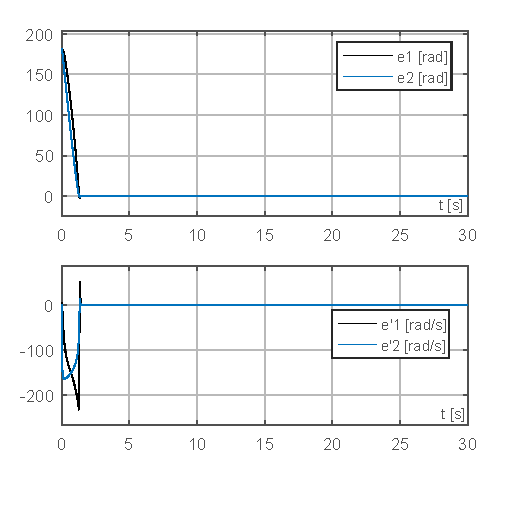
\includegraphics[width=0.30\columnwidth]{SRManL4_ZADANIE2/figs/02Uchyby_U24} c)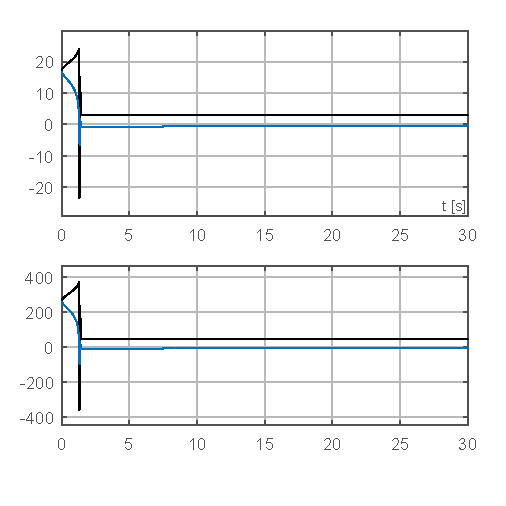
\includegraphics[width=0.30\columnwidth]{SRManL4_ZADANIE2/figs/02Sygnaly_U24}\caption{
			Wyniki symulacji dla $u_{HKmax}=24$ [V]. Przebiegi a) pozycji ogniw wraz z zadanym sygnałem referencyjnym, b) uchybów pozycji i prędkości, c)  napięć sterujących oraz odpowiadające im momenty generowane na wałach silników, o wymuszeniu: $Q_d=[1\quad1]$}
	\end{figure}


\end{document}
